\documentclass[conference]{IEEEtran}
\IEEEoverridecommandlockouts
% The preceding line is only needed to identify funding in the first footnote. If that is unneeded, please comment it out.
\usepackage{cite}
\usepackage{amsmath,amssymb,amsfonts}
\usepackage{algorithmic}
\usepackage{graphicx}
\usepackage{textcomp}
\usepackage{xcolor}
\usepackage{enumitem}
\usepackage{array}
\def\BibTeX{{\rm B\kern-.05em{\sc i\kern-.025em b}\kern-.08em
		T\kern-.1667em\lower.7ex\hbox{E}\kern-.125emX}}
\bibliographystyle{plain}
\begin{document}
	
	\title{Analisis Perbandingan Performa Pola Arsitektur MVC dan MVVM dalam Mengeksekusi Operasi\\
		{\footnotesize \textsuperscript{}}
		\thanks{}
	}
	
	\author{\IEEEauthorblockN{Andrew Kurniawan Gianto}
		\IEEEauthorblockA{\textit{Informatika} \\
			\textit{Pradita University}\\
			Tangerang, Indonesia \\
			andrew.kurniawan@student.pradita.ac.id}
		\and
		\IEEEauthorblockN{Ryo Ferdinand}
		\IEEEauthorblockA{\textit{Informatika} \\
			\textit{Pradita University}\\
			Tangerang, Indonesia \\
			ryo.ferdinand@student.pradita.ac.id}
		\and
		\IEEEauthorblockN{Eka Rifail Saipuddin Rachman}
		\IEEEauthorblockA{\textit{Informatika} \\
			\textit{Pradita University}\\
			Tangerang, Indonesia \\
			eka.rifail@student.pradita.ac.id}
		\and
		\and
		\and
		\IEEEauthorblockN{Verrel Novendra Sulu}
		\IEEEauthorblockA{\textit{Informatika} \\
			\textit{Pradita University}\\
			Tangerang, Indonesia \\
			verrel.novendra@student.pradita.ac.id}
		\and
		\and
		\and
		\and
		\and
		\and
		\IEEEauthorblockN{Hezel Anthonie Norman Piter Papia}
		\IEEEauthorblockA{\textit{Informatika} \\
			\textit{Pradita University}\\
			Tangerang, Indonesia \\
			hezel.anthonie@student.pradita.ac.id}
	}
	
	\maketitle
	
	\begin{abstract}
		Pemilihan model arsitektur yang tepat sangat penting untuk mengembangkan aplikasi. Seiring berkembangnya teknologi, para pengembang harus memahami model arsitektur yang akan digunakan untuk mengembangkan aplikasi. Penelitian ini bertujuan untuk membandingkan dua model arsitektur perangkat lunak, yaitu \textit{Model-View-Controller}(MVC) dan \textit{Model-View-ViewModel}(MVVM). 
		
		Tahap penelitian ini terbagi menjadi 5 tahap, yaitu Identifikasi Masalah, Pengumpulan Data, Perancangan, Implementasi, dan Pengujian. Pada tahap Identifikasi Masalah, menentukan model arsitektur yang lebih baik dalam beberapa aspek akan dilakukan.  Pada tahap Pengumpulan Data, penting mengumpulkan data-data untuk membandingkan kedua model arsitektur. Pada tahap Perancangan, class diagram dan sequence diagram kedua arsitektur dirancang untuk menemukan kedua pola arsitektur. Pada tahap Implementasi, kedua kode arsitektur diterapkan berdasarkan class diagram dan sequence diagram yang telah dirancang. Pada tahap Pengujian, pola arsitektur MVC dan MVVM akan diuji.
		
		Testing aplikasi dibutuhkan untuk menghasilkan 4 aspek, yaitu \textit{View to total time, View to total memory, Spin to total time,} dan \textit{Spin to total memory}. Dengan adanya hasil dari 4 aspek tersebut, kita dapat mengetahui arsitektur model manakah yang lebih unggul.
		
		
	\end{abstract}
	
	\begin{IEEEkeywords}
		MVC, MVVM, kecepatan, \textit{memory}, \textit{Spin, View}
	\end{IEEEkeywords}
	
	\section{Pendahuluan}
	
	Perangkat lunak telah menjadi dasar bagi banyak aplikasi dan sistem yang digunakan dalam berbagai aspek kehidupan di era teknologi informasi yang terus berkembang. Perangkat lunak telah mendominasi cara kita berinteraksi dengan dunia digital. Dari infrastruktur bisnis yang membantu operasi perusahaan hingga aplikasi yang memenuhi kebutuhan sehari-hari. Tanpa adanya perangkat lunak yang efektif dan terorganisir, akses dalam bertransaksi, berkomunikasi, dan memperoleh informasi akan terbatas. Perangkat lunak telah mengubah cara kita bekerja, bermain, dan juga berinteraksi dengan dunia luar.  Oleh karena itu, perangkat lunak tidak hanya harus beroperasi dengan efisien, tetapi juga harus mudah dikembangkan dan diubah sesuai kebutuhan. Pengembang perangkat lunak dituntut untuk menulis kode yang mudah dipahami dan dikelola, terutama untuk sistem yang kompleks dengan masalah yang berulang.
	
	Pola desain antarmuka pengguna dapat membantu mengurangi kekacauan dalam sistem yang kompleks, membuat aplikasi lebih terorganisir dan dapat diskalakan. Dengan mempelajari dan menerapkan pola antarmuka pengguna yang tepat, pengembang dapat membuat aplikasi yang lebih efisien dan terstruktur. Pola arsitektur ini dapat memungkinkan pengembang untuk fokus pada masalah yang spesifik. Saat ini, ada berbagai macam pola arsitektur pengembang yang masing-masing arsitektur memiliki kelebihan dan kekurangan sehingga tidak semua arsitektur cocok dalam segala hal. Karena itu, memilih arsitektur yang tepat sangat penting bagi pengembang untuk memastikan aplikasi yang dikembangkan dapat memenuhi kebutuhan pengguna. Dalam artikel ini, akan dibahas dua arsitektur populer, yaitu \textit{Model-View-Controller} (MVC) dan \textit{Model-View-ViewModel} (MVVM).
	
	Tujuan dari penelitian ini adalah untuk membandingkan kinerja arsitektur MVC dengan MVVM, khususnya dalam hal kecepatan dan penggunaan memori. MVC telah lama menjadi arsitektur yang umum digunakan dalam pengembangan perangkat lunak, terutama dengan pendekatan prototipe. Di sisi lain, MVVM sering digunakan dalam pengembangan aplikasi mobile. Penelitian ini akan menentukan arsitektur mana yang paling efisien dan sesuai dengan berbagai kebutuhan pengembangan perangkat lunak melalui eksperimen yang berfokus pada komponen \textit{Model-View} (MV).
	
	Hasil dari penelitian ini diharapkan dapat membantu pengembang perangkat lunak memahami kelebihan dan kelemahan masing-masing arsitektur, serta menambah wawasan tentang performa masing-masing arsitektur. Meskipun kedua arsitektur ini telah populer sebagai pengembangan perangkat lunak, pengembang perlu memahami dengan lebih baik mengenai kinerja dan karakteristik masing-masing arsitektur. Dengan demikian, pengembang dapat mengurangi risiko pengembangan dengan membuat keputusan yang lebih baik dalam memilih arsitektur yang tepat untuk proyek mereka, menghasilkan aplikasi yang lebih baik, efisien, dan andal di era teknologi informasi yang terus berkembang.
	
	
	\section{Kajian Terkait}
	
	\subsection{Model-View-Controller (MVC)}
	\textit{Model-View-Controller} atau MVC adalah arsitektur perangkat lunak untuk membuat sebuah aplikasi dengan memisahkan data (\textit{Model}) dari tampilan (\textit{View}) dan cara bagaimana memprosesnya (\textit{Controller})\cite{Perbandingan4} \cite{MVC} . MVC menekankan tiga elemen penting: perhatian, tanggung jawab, dan logika. Ini mempercepat kinerjanya.
	
	Penjelasan dari masing-masing komponen MVC dapat dilihat pada figure 1, dan mempunyai penjelasan sebagai berikut:
	\begin{enumerate}[label=\alph*]
		\item Bagian \textit{model} biasanya digunakan untuk mengambil data dari database atau menyimpan data ke dalam database. 
		\item Bagian \textit{view} adalah komponen yang menampilkan antarmuka pengguna aplikasi, yang dibangun berdasarkan data model. 
		\item Bagian \textit{control} adalah bagian yang menangani interaksi pengguna, bekerja dengan model, dan menyimpan data ke dalam database.
	\end{enumerate}
	
	\begin{figure}[h]
		\centering
		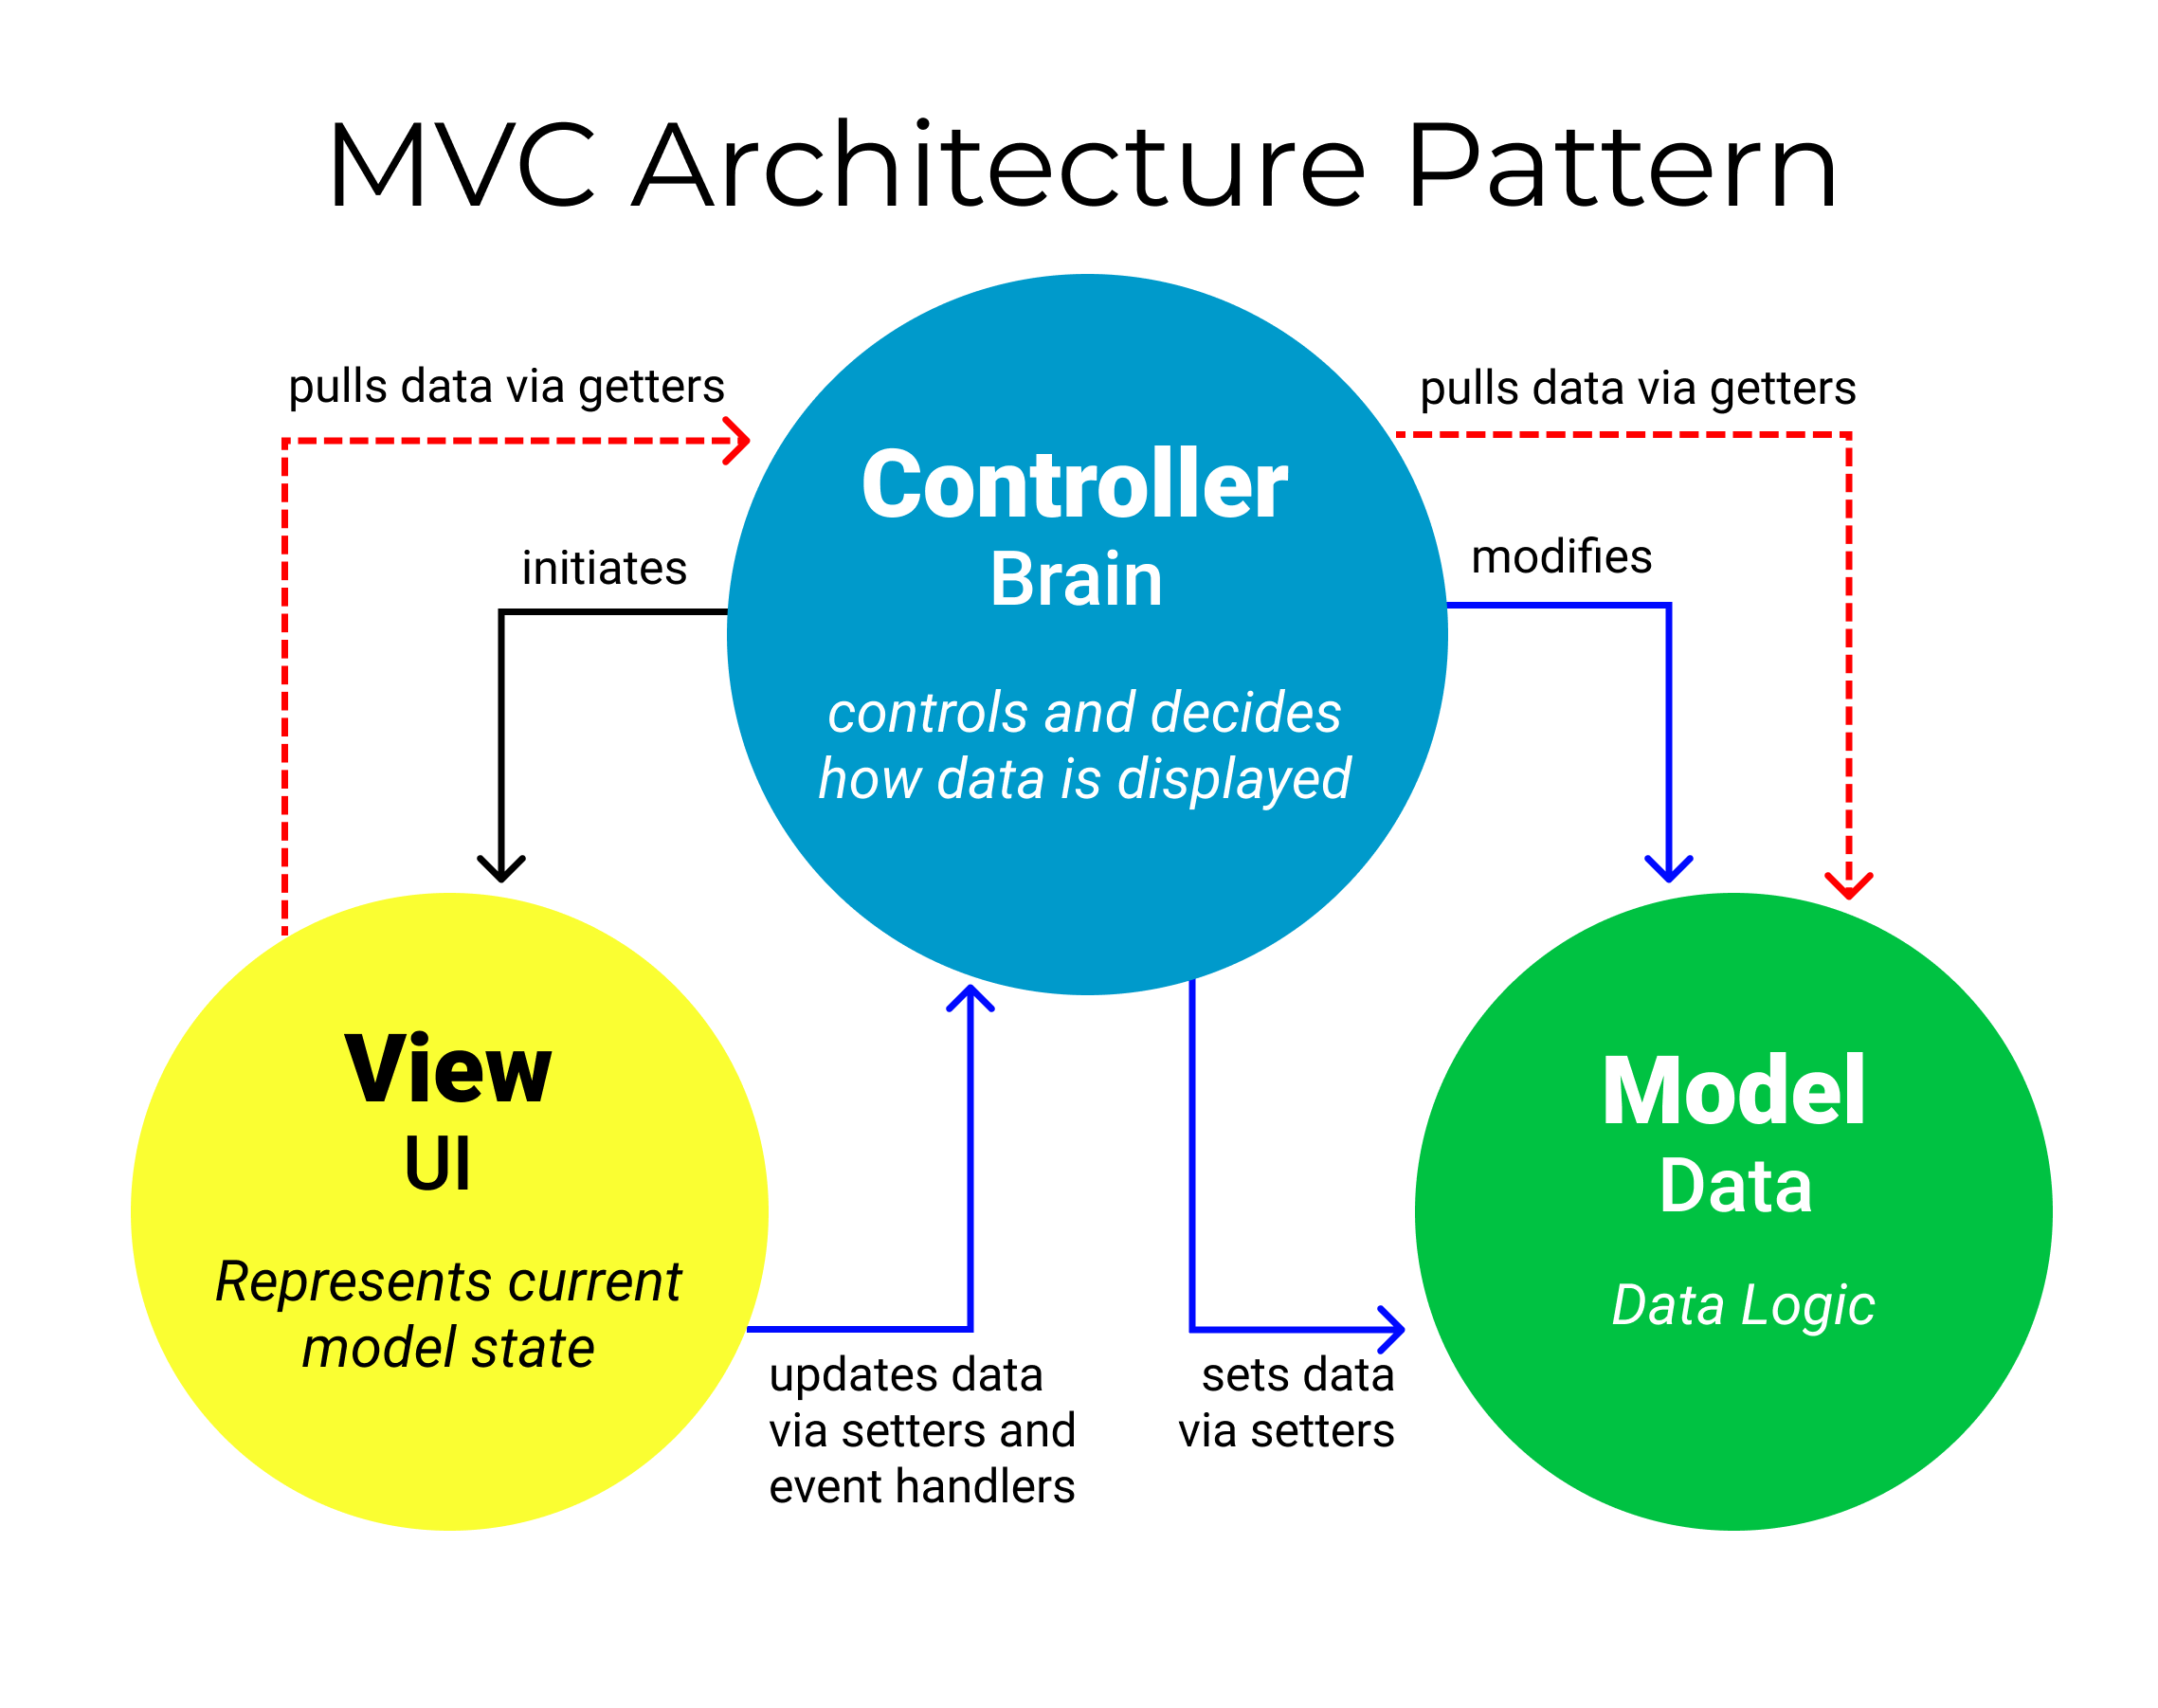
\includegraphics[width=0.5\textwidth]{images/MVC3}
		\caption{Arsitektur MVC}
		\label{fig:class_mvvm}
	\end{figure}
	
	Penjelasan mengenai keuntungan dan kerugian dari arsitektur MVC adalah sebagai berikut:
	\subsubsection{Keuntungan}
	\begin{itemize}
		\item Pemisahan tanggung jawab antara \textit{Model, View,} dan \textit{Control} membuat aplikasi lebih mudah dipahami, diuji, dan dikembangkan.
		\item Fleksibilitas dalam mengganti atau memodifikasi salah satu komponen tanpa memengaruhi komponen lainnya.
		\item Memungkinkan pengembangan paralel antara komponen-komponen aplikasi.
	\end{itemize}
	\subsubsection{Kerugian}
	\begin{itemize}
		\item Adanya kompleksitas dalam pengelolaan koneksi antara 3 komponen tersebut.
		\item Adanya kesulitan dalam pengujian unit pada \textit{View} dan \textit{Controller}.
	\end{itemize}
	
	\subsection{Model-View-View-Model (MVVM)}
	\textit{Model View ViewModel} (MVVM) adalah sebuah arsitektur perangkat lunak yang memisahkan antara kode untuk logika bisnis dan tampilan aplikasi\cite{MVVM}. Dalam kata lain, MVVM adalah sebuah pattern desain yang terdiri dari tiga komponen: \textit{Model, View, dan ViewModel} \cite{MVVM2}.  
	
	Penjelasan dari masing-masing komponen MVVM dapat dilihat pada figure 2, dan mempunyai penjelasan sebagai berikut:
	\begin{enumerate}[label=\alph*]
		\item Bagian \textit{model} merupakan representasi dari data yang digunakan dalam logika bisnis.
		\item Bagian \textit{view} adalah komponen yang terdiri dari layout sumber daya file dan aktivitas/fragmen. Activity/Fragment secara dinamis mengontrol tampilan pada layout sumber daya file.
		\item Bagian \textit{ViewModel} berinteraksi dengan Model dan menyiapkan variabel yang akan diamati oleh \textit{View}. \textit{ViewModel} bersifat lifecycle-aware, sehingga kelas ini akan hidup ketika sebuah kelas View telah melalui tahapan create dan belum melalui tahapan destroy.
	\end{enumerate}
	
	\begin{figure}[h]
		\centering
		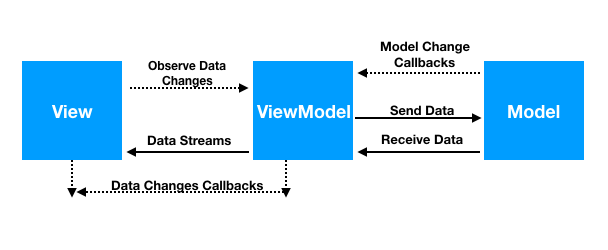
\includegraphics[width=0.5\textwidth]{images/MVVM}
		\caption{Arsitektur MVVM}
		\label{fig:class_mvvm}
	\end{figure}
	
	Penjelasan mengenai keuntungan dan kerugian dari arsitektur MVVM adalah sebagai berikut:
	\subsubsection{Keuntungan}
	\begin{itemize}
		\item Pemisahan antara \textit{View} dan \textit{ViewModel} sehingga membuat pengujian dan pemeliharaan kode lebih mudah
		\item Kode MVVM biasanya digerakkan oleh peristiwa, yang berarti kode dapat diuji secara terpisah.
	\end{itemize}
	\subsubsection{Kerugian}
	\begin{itemize}
		\item Komponen antarmuka MVVM harus dibuat observable yang berarti dapat memakan waktu dan rumit.
		\item Banyak kode yang harus ditulis dan dikelola untuk setiap komponen UI sehingga aplikasi dapat menjadi lebih sulit untuk digunakan dan dipahami.
	\end{itemize}
	
	\subsection{Studi Preseden}
	Dalam penelitian "Perbandingan Kinerja Pola Perancangan MVC, MVP, dan MVVM Pada Aplikasi Berbasis Android (Studi Kasus: Aplikasi Laporan Hasil Belajar Siswa SMA BSS)"\cite{Perbandingan1}, dibahas analisis perbandingan tiga pola perancangan arsitektur perangkat lunak yang populer: Model-View-Controller, Model-View-Presenter, dan Model-View-ViewModel (MVVM). Aplikasi laporan hasil belajar siswa SMA Brawijaya Smart School digunakan sebagai basis untuk penelitian ini. Tujuan dari penelitian ini adalah untuk menemukan pola perancangan yang paling hemat energi dan memori untuk aplikasi Android. Penelitian dimulai dengan rekayasa untuk menentukan persyaratan fungsional dan non-fungsional. Persyaratan ini kemudian digunakan sebagai dasar untuk desain dan pelaksanaan penelitian. Ketiga pola desain ini digunakan untuk memulai implementasi Java. Setelah tahap implementasi, setiap aplikasi yang menggunakan pola ini diuji. Pengujian dilakukan sebanyak lima kali untuk mendapatkan data penggunaan energi dan memori. Hasil pengujian menunjukkan bahwa ketiga pola perancangan memiliki penggunaan energi yang sederhana, dengan penggunaan memori rata-rata 59,7 MB untuk MVC, 59 MB untuk MVP, dan 73,2 MB untuk MVVM. Selain itu, tahap pengujian fungsional dengan metode pengujian blackbox memberikan hasil validitas sebesar 100\% untuk semua fungsi.
	
	\begin{table}[ht]
		\centering
		\caption{Perbandingan Memori dan Waktu Eksekusi Berdasarkan penelitian ”Perbandingan Kinerja Pola Perancan-
			gan MVC, MVP, dan MVVM Pada Aplikasi Berbasis Android"}
		\label{tab:comparison}
		\begin{tabular}{|l|l|}
			\hline
			\textbf{Arsitektur} & \textbf{Penggunaan Memori (MB)} \\ \hline
			MVC & 59.7 \\ \hline
			MVP & 59.0 \\ \hline
			MVVM & 73.2 \\ \hline
		\end{tabular}
	\end{table}
	
	
	Dalam penelitian "A Comparison of Android Native App Architecture—MVC, MVP, and MVVM"\cite{Perbandingan2}, dibahas mengenai masalah efisiensi dan kualitas pengembangan aplikasi Android yang dipengaruhi oleh arsitektur aplikasi. Tujuan dari artikel ini adalah untuk memberikan analisis menyeluruh untuk menentukan apakah arsitektur MVP (Model-View-Presenter) dan MVVM (Model-View-ViewModel) lebih unggul dari arsitektur aplikasi Android native bawaan, yaitu MVC (Model-View-Controller). Dengan menggunakan Metode Analisis Tradeoff Arsitektur untuk menjawab pertanyaan ini dan menetapkan tiga kriteria: ketepatan, modifikasi, dan kinerja. Berdasarkan kriteria ini, mereka mengenali faktor-faktor penting untuk setiap atribut kualitas dan melakukan perbandingan. Hasil analisis dan eksperimen menunjukkan bahwa MVP dan MVVM lebih unggul daripada MVC dalam hal testability, modifiability (tingkat coupling yang rendah), dan performance (mengonsumsi memori yang lebih sedikit).
	
	Dalam penelitian "Performance Comparison of Native Android Application on MVP and MVVM"\cite{Perbandingan3}, dibahas analisis komparatif terhadap arsitektur MVP (\textit{Model-View-Presenter}) dan MVVM (\textit{Model-View-ViewModel}) dalam konteks pengembangan aplikasi Android asli dilakukan dalam makalah yang ditulis oleh Wisnuadhi, Munawar, dan Wahyu. Tujuan dari penelitian ini adalah untuk mengevaluasi kinerja kedua arsitektur tersebut dengan mempertimbangkan tiga faktor: penggunaan CPU, penggunaan memori, dan waktu eksekusi. Hasil eksperimen menunjukkan bahwa arsitektur MVVM lebih baik dalam penggunaan CPU dan waktu eksekusi, sedangkan MVP unggul dalam penggunaan memori. Aplikasi MVVM memiliki penggunaan CPU yang lebih rendah dengan perbedaan rata-rata 0,55\% dan waktu eksekusi yang lebih cepat dengan perbedaan rata-rata 126,21 ms. Aplikasi MVP juga memiliki penggunaan memori yang lebih rendah dengan perbedaan rata-rata 0,92 MB.
	
	\begin{table}[ht]
		\centering
		\caption{Perbandingan Penggunaan Memori dan Waktu Eksekusi Berdasarkan penelitian "Performance Comparison of Native Android Application on MVP and MVVM"}
		\label{tab
		}
		\begin{tabular}{|l|l|l|}
			\hline
			\textbf{Arsitektur} & \textbf{Waktu Eksekusi} \\ \hline
			MVP & lebih pelan 126,21 ms\\ \hline
			MVVM & lebih cepat 126,21 ms \\ \hline
		\end{tabular}
	\end{table}
	\section{Metodologi}
	Metodologi penelitian ini terbagi menjadi 5 tahap, yaitu Tahap Identifikasi Masalah, Tahap Pengumpulan Data, Tahap Perancangan, Tahap Implementasi, dan terakhir Tahap Pengujian.
	\subsection{Identifikasi Masalah}
	Masalah utama penelitian ini adalah untuk menentukan model arsitektur mana yang lebih baik dan cepat dalam empat aspek utama: penggunaan memori total saat melakukan operasi spin, waktu total yang dibutuhkan untuk melakukan operasi spin, penggunaan memori total saat melakukan operasi pandang, dan waktu total yang dibutuhkan untuk melakukan operasi pandang. Pemilihan arsitektur yang tepat sangat penting untuk memastikan bahwa sebuah aplikasi dapat beroperasi dengan efisien daripada sebelumnya. Perbandingan model arsitektur dalam penelitian ini adalah membandingkan kinerja arsitektur \textit{Model-View-Controller} (MVC) dan \textit{Model-View-ViewModel} (MVVM) dalam halnya kecepatan dan penggunaan memori.
	
	\subsection{Pengumpulan Data}
	Mengumpulkan data-data tentang arsitektur MVC dan MVVM penting untuk mendapatkan dasar teoritis dan pemahaman yang kuat. Dimulai dari membaca literatur yang ada tentang topik tersebut untuk memahami konsep dasar, manfaat, dan kelemahan dari masing-masing arsitektur. Kemudian mengumpulkan studi kasus yang relevan yang memberikan penjelasan teoritis dan aplikasi praktis dari arsitektur MVC dan MVVM dalam berbagai konteks. Studi kasus ini juga memberikan wawasan penting tentang bagaimana arsitektur ini digunakan dan diimplementasikan dalam situasi tertentu.
	
	\subsection{Perancangan}
	Untuk mendapat gambaran mengenai pola arsitektur untuk setiap \textit{model} (MVC dan MVVM) yang lebih jelas, kami merancang class diagram dan sequence diagram untuk kedua arsitektur \textit{model} tersebut. Untuk memastikan representasi yang jelas dan konsisten dari masing-masing arsitektur, diagram ini dibuat menggunakan kode PlantUML. 
	
	\subsubsection{Pola Arsitektur MVC}
	\paragraph{Class Diagram}
	Class diagram \textit{Model-View-Controller} (MVC), pada figure 3, menggambarkan tiga komponen utama yang berkolaborasi untuk memisahkan logika bisnis dari tampilan antarmuka pengguna. Komponen pertama adalah \textit{Model}, yang bertanggung jawab untuk mengelola data dan logika bisnis. \textit{Model} mengakses basis data atau sumber data lainnya, melakukan operasi seperti perhitungan, dan mengirimkan data ke komponen lain seperti \textit{controller} atau \textit{view}. Komponen kedua adalah \textit{View}, yang bertugas menampilkan data kepada pengguna. \textit{View} mengambil data dari \textit{model} dan menampilkannya dalam format yang sesuai, seperti antarmuka pengguna grafis atau laporan teks. Komponen ketiga adalah \textit{Controller}, yang berfungsi sebagai penghubung antara \textit{model} dan \textit{view}. \textit{Controller} menerima input dari pengguna melalui view, memprosesnya (yang mungkin melibatkan interaksi dengan model), dan menentukan \textit{view} mana yang harus diperbarui dengan data terbaru. Class Diagram MVC menampilkan hubungan ini dengan jelas: \textit{model} dan \textit{view} berinteraksi dengan \textit{controller}, yang mengatur aliran data di antara keduanya.
	
	\begin{figure}[h]
		\centering
		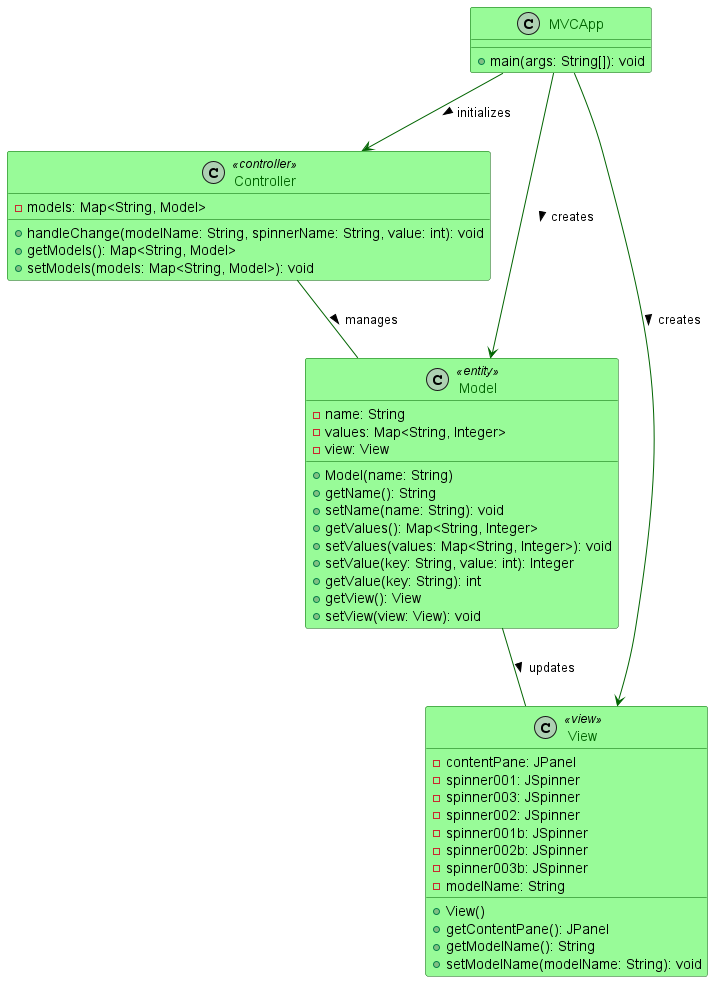
\includegraphics[width=0.3\textwidth]{../Class_Sequence_Diagram/out/MVC_ClassDiagram/MVC_ClassDiagram}
		\caption{Class Diagram MVC}
		\label{fig:Class_mvc}
	\end{figure}
	
	\vspace{1cm}
	
	\paragraph{Sequence Diagram}
	Sequence diagram  MVC, seperti yang diilustrasikan figure 4, menggambarkan alur interaksi antara pengguna, \textit{view, controller}, dan \textit{model} dalam skenario operasi umum. Ketika pengguna memasukkan input ke dalam \textit{view, view} meneruskan input tersebut ke \textit{controller. Controller} kemudian memproses input ini dan memperbarui \textit{model} dengan data baru. Setelah \textit{model} diperbarui, \textit{controller} meminta \textit{view} untuk memperbarui tampilannya berdasarkan data terbaru dari \textit{model}. Akhirnya, \textit{view} menampilkan data terbaru kepada pengguna. Proses ini menggambarkan bagaimana MVC memisahkan tanggung jawab di antara komponen-komponennya untuk menjaga modularitas dan skalabilitas aplikasi.
	
	
	\begin{figure}[h]
		\centering
		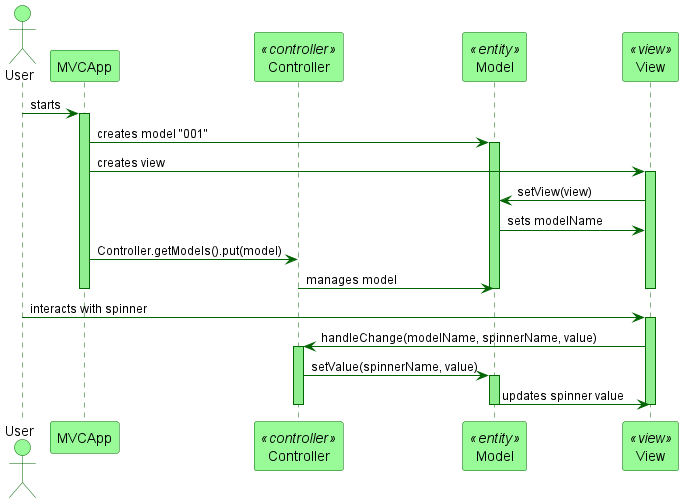
\includegraphics[width=0.4\textwidth]{../Class_Sequence_Diagram/out/MVC_SequenceDiagram/MVC_SequenceDiagram}
		\caption{Sequence Diagram MVC}
		\label{fig:Sequence_mvc}
	\end{figure}
	
	
	\subsubsection{Pola Arsitektur MVVM}
	\paragraph{Class Diagram}
	Dalam Class Diagram \textit{Model-View-ViewModel} (MVVM) yang ada pada figure 5, terdapat hubungan antara tiga komponen utama yang dirancang untuk mendukung data binding dan memisahkan logika UI dari logika bisnis. \textit{Model} dalam MVVM bertanggung jawab untuk data dan logika bisnis, sama seperti dalam MVC. \textit{View} bertanggung jawab untuk menampilkan data kepada pengguna, namun dalam MVVM, \textit{view} lebih terikat erat dengan \textit{ViewModel} melalui mekanisme data \textit{binding}. \textit{ViewModel} adalah komponen yang berfungsi sebagai penghubung antara \textit{view} dan \textit{model}. \textit{ViewModel} mengambil data dari \textit{model}, mengolahnya jika perlu, dan menyediakan data yang diformat untuk \textit{view}. \textit{ViewModel} juga menangani logika UI yang diperlukan oleh \textit{view}, memungkinkan \textit{view} untuk tetap sederhana dan fokus pada rendering antarmuka.
	
	\begin{figure}[h]
		\centering
		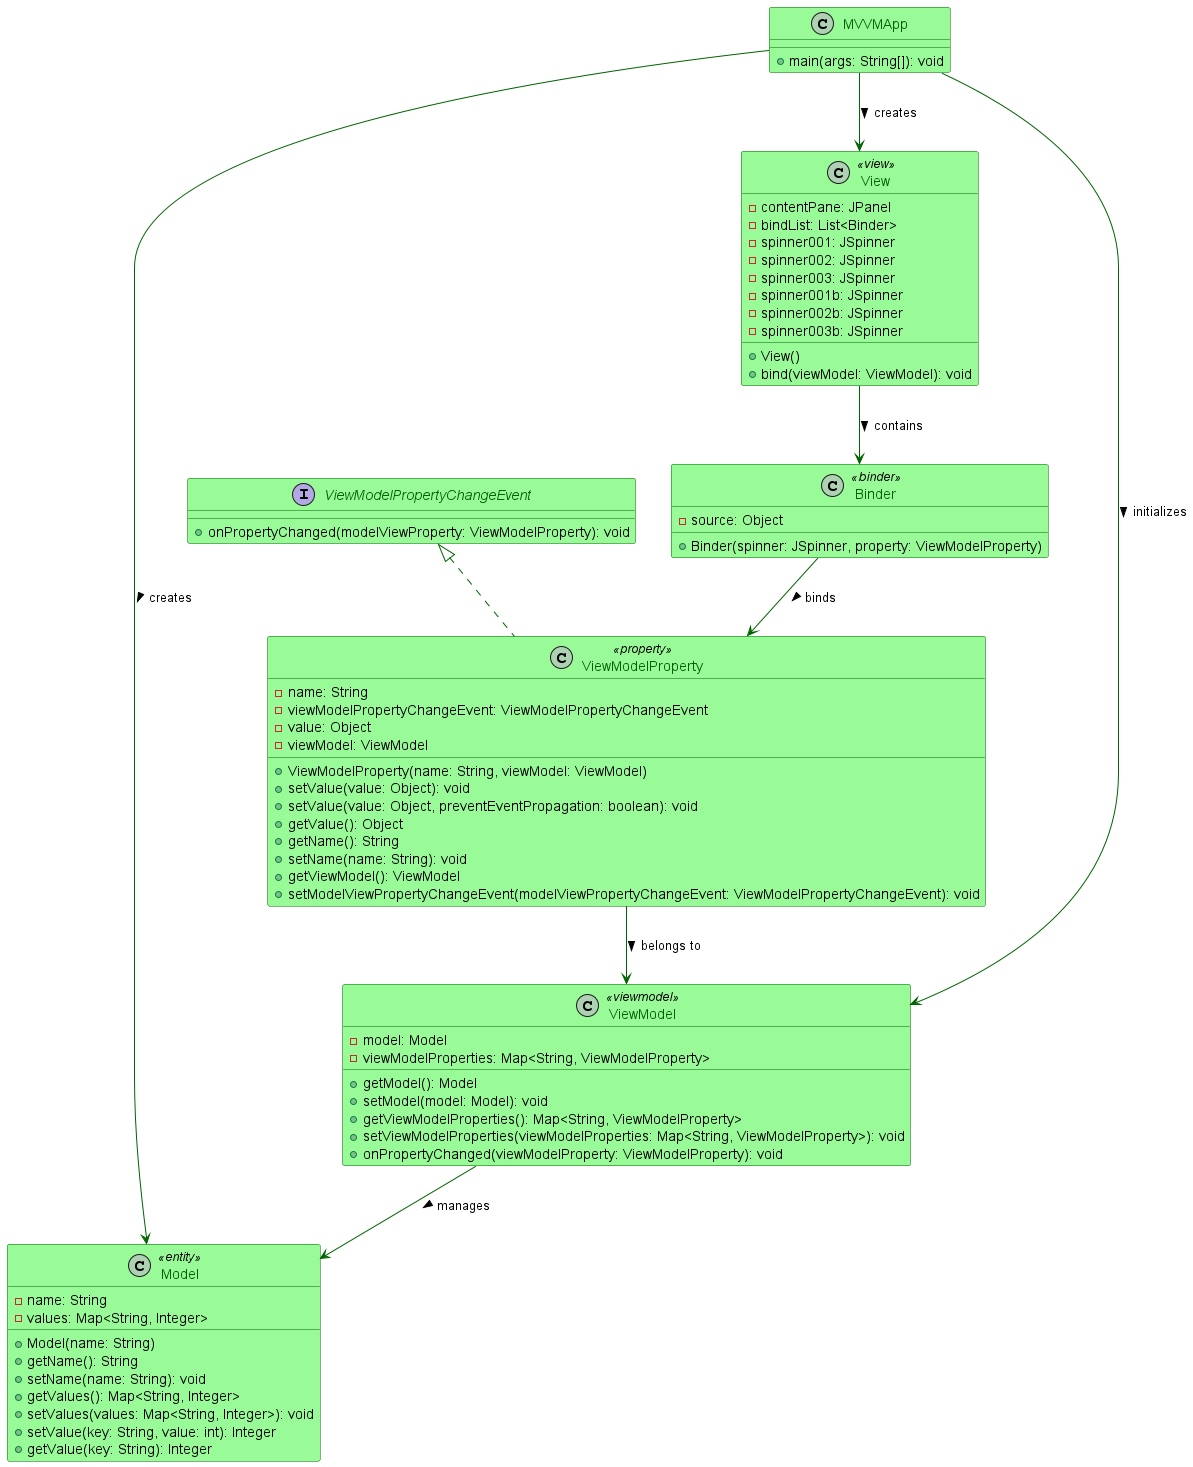
\includegraphics[width=0.3\textwidth]{../Class_Sequence_Diagram/out/MVVM_ClassDiagram/MVVM_ClassDiagram}
		\caption{Class Diagram MVVM}
		\label{fig:Class_MVVM}
	\end{figure}
	
	\vspace{5cm}
	
	\paragraph{Sequence Diagram}
	Sequence diagram MVVM, seperti yang diilustrasikan pada figure 6, menggambarkan alur interaksi antara pengguna, \textit{view, ViewModel}, dan \textit{model} dalam skenario operasi umum. Ketika pengguna memasukkan input ke dalam \textit{view}, input tersebut dikirim ke \textit{ViewModel}. \textit{ViewModel} memproses input ini dan memperbarui \textit{model} sesuai dengan data yang baru. \textit{Model} kemudian memperbarui datanya. Setelah \textit{model} diperbarui, \textit{ViewModel} mengambil data terbaru dari \textit{model} dan memperbarui data yang terikat pada \textit{view}. \textit{View} kemudian menampilkan data terbaru kepada pengguna. Proses ini menunjukkan bagaimana MVVM memanfaatkan data \textit{binding} untuk mengelola aliran data antara \textit{model} dan \textit{view} melalui \textit{ViewModel}, memudahkan pengembangan dan pemeliharaan antarmuka pengguna yang dinamis dan responsif.
	
	\begin{figure}[h]
		\centering
		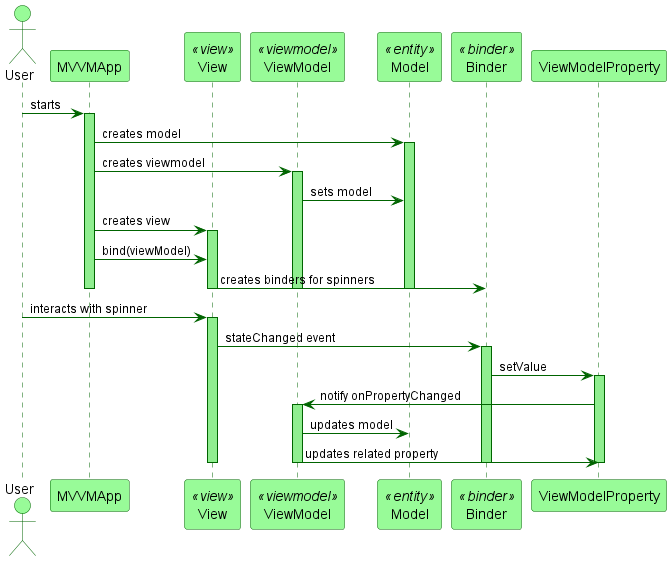
\includegraphics[width=0.4\textwidth]{../Class_Sequence_Diagram/out/MVVM_SequenceDiagram/MVVM_SequenceDiagram}
		\caption{Sequence Diagram MVVM}
		\label{fig:Sequence_MVVM}
	\end{figure}
	
	\subsection{Implementasi}
	Dalam tahap implementasi ini, ada penerapan kode untuk kedua arsitektur (MVC dan MVVM) berdasarkan class diagram dan sequence diagram yang sudah dirancang. Implementasi kode MVC melibatkan pembuatan kelas \textit{model, view}, dan \textit{controller} sesuai dengan Class Diagram yang telah dirancang. Pada implementasi kode MVVM, kami membuat kelas \textit{model, view}, dan \textit{viewmodel} serta \textit{binder} untuk menghubungkan \textit{view} dengan \textit{viewmodel properties}. Kode yang diimplementasikan lalu akan diuji dalam TestApp masing-masing \textit{model} arsitektur. Source code tersebut terlihat pada figure 7.
	
	\begin{figure}[h]
		\centering
		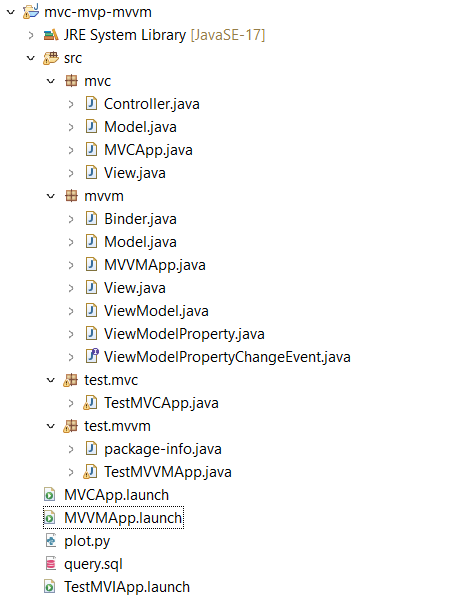
\includegraphics[width=0.3\textwidth]{images/ImplementasiKode}
		\caption{Source Code mvc-mvvm}
		\label{fig:mvc_mvvm}
	\end{figure}
	
	\subsubsection{Pola Arsitektur MVC}
	\textit{Model-View-Controller} (MVC) terdiri dari: \textit{Model}, \textit{View}, \textit{Controller}, dan \textit{MVCApp}. Masing-masing file memiliki tugas khusus yang berkontribusi terhadap keseluruhan arsitektur MVC.
	
	File \textit{Model} berfungsi untuk menyimpan data aplikasi, memanipulasi data, dan mengubah tampilan komponen di \textit{view} berdasarkan perubahan data. 
	
	File \textit{View} berfungsi untuk menampilkan data, menerima input dari pengguna dan mengirimkan perubahan ke \textit{controller}, dan menghubungkan \textit{view} dengan \textit{model} untuk memperbarui tampilan berdasarkan perubahan data. 
	
	File \textit{Controller} berfungsi untuk menerima input dari \textit{view} dan memprosesnya, memperbarui data di \textit{model} berdasarkan input yang diterima, menyimpan dan mengelola beberapa \textit{model} dalam aplikasi. 
	
	File MVCApp berfungsi untuk menyiapkan \textit{model, view}, dan \textit{controller}, menghubungkan \textit{model} dengan \textit{view} dan \textit{controller}, dan menjalankan aplikasi dengan menampilkan \textit{view} kepada pengguna. 
	
	\subsubsection{Pola Arsitektur MVVM}
	Model-View-ViewModel (MVVM) memiliki tujuh file: \textit{Binder, Model, View, ViewModel, ViewModelProperty, ViewModelPropertyChangeEvent,} dan \textit{MVVMApp}. 
	
	File \textit{Binder} berfungsi untuk menghubungkan JSpinner dengan \textit{ViewModelProperty}, \textit{Binder} memungkinkan komunikasi dua arah antara komponen GUI dengan logika aplikasi dalam arsitektur MVVM.
	
	File \textit{Model} bertanggung jawab untuk menyimpan dan mengelola data yang dibutuhkan oleh aplikasi.
	
	File \textit{View} berfungsi untuk menampilkan antarmuka kepada pengguna serta memfasilitasi interaksi antara pengguna dan aplikasi.
	
	File \textit{ViewModel} berfungsi untuk mengelola data yang diperlukan oleh \textit{View} dan melakukan komunikasi dengan \textit{View} dan \textit{Model}, file \textit{ViewModel} juga bertanggung jawab untuk menjaga konsistensi data antara \textit{Model} dan \textit{View}. 
	
	File \textit{ViewModelProperty} berfungsi untuk merepresentasikan data atau properti dalam \textit{ViewModel}.
	
	File \textit{ViewModelPropertyChangeEvent} berfungsi untuk menangani apabila terjadi adanya perubahan pada nilai dengan cara memperbarui tampilan yang terkait dengan perubahan nilai tersebut. 
	
	File MVVMApp berfungsi untuk menjalankan aplikasi dan mengatur pembuatan dan konfigurasi 
	komponen MVVM yaitu \textit{Model, ViewModel} dan \textit{View}. Aplikasi ini memungkinkan sinkronisasi antara data dan antarmuka pengguna sehingga memudahkan pengelolaan.
	
	\subsection{Pengujian}
	Dalam tahap pengujian ini, kami menguji kedua pola arsitektur (MVC dan MVVM) pada TestApp masing-masing. Setiap model akan mempunyai 10 instance dan setiap instance ini memiliki \textit{view} yang berisi jumlah JSpinner yang berbeda. Instance pertama (\textit{View} 1) hanya berisi 1 JSpinner, instance kedua (\textit{View} 2) berisi 2 JSpinner, dan seterusnya hingga instance ke-100 (\textit{View} 100) yang berisi 100 JSpinner. Dalam setiap eksperimen, semua nilai JSpinner dari \textit{View} 1 hingga \textit{View} 100 akan diubah, dan waktu yang dibutuhkan untuk menyelesaikan operasi ini akan direkam. Eksperimen ini akan diulang sebanyak 12 kali untuk memastikan konsistensi dan reliabilitas hasil. Testing yang dijalankan akan mengeluarkan output \textit{iteration, view total, view num, spin total, spin num, time, memory}. Begitu juga ada konfigurasi untuk total view dan spinner (1, 25, 50, 75, 100). Output tersebut lalu akan disimpan pada file data.csv masing-masing model. Hasil dari pengujian lalu akan digunakan untuk membandingkan penggunaan memori dan waktu eksekusi antara MVC dan MVVM. 
	\subsubsection{Testing Pola Arsitektur MVC}
	Cara kerja TESTMVCApp adalah \textit{View} akan mendeteksi data yang dimasukkan pada input spinner lalu mengirimkan data tersebut ke \textit{controller}. \textit{Controller} akan menerima data tersebut dan akan mencari \textit{model} yang sesuai dengan \textit{model} yang diterima dari \textit{view}. Setelah menemukan \textit{model} yang sesuai, \textit{controller} akan mengubah data tersebut. Lalu \textit{model} akan mengubah tampilan pada \textit{view} sehingga pengguna dapat melihat data yang baru. Program akan mengulang proses pengukurannya sebanyak 12 kali. Setiap hasil pengukuran yang telah dilakukan akan disimpan di dalam file MVCdata.csv yang baru dibuat program.
	\subsubsection{Testing Pola Arsitektur MVVM}
	Cara kerja TESTMVVMApp adalah \textit{model} menyimpan data, \textit{ViewModel} bertindak sebagai mediator yang menghubungkan \textit{Model} dengan \textit{View}, dan \textit{View} menampilkan data serta memperbarui dirinya berdasarkan perubahan yang terjadi di \textit{ViewModel}, dengan \textit{binding} ini memungkinkan untuk \textit{View} memperbarui secara otomatis ketika data pada \textit{ViewModel} berubah. Input \textit{spinner} di \textit{View} ditambahkan yang akan mengubah data di \textit{ViewModel} dan kemudian diperbarui secara otomatis di \textit{View} melalui \textit{binding}. Program lalu akan menjalankan looping proses measurementnya sebanyak 12 kali. Pada setiap iterasi, program membuat dan mengatur hubungan antara \textit{Model}, \textit{ViewModel}, dan \textit{View}. Setiap \textit{View} dibuat dengan sejumlah \textit{spinner} input dan output yang sesuai dengan jumlah yang ditentukan. \textit{Spinner} input terhubung dengan listener yang memperbarui data di \textit{ViewModel}, yang kemudian menggandakan nilai input dan memperbarui \textit{spinner} output. Setelah semua \textit{View} dibuat dan \textit{spinner} diatur, program mencatat data performa, seperti jumlah \textit{view}, jumlah \textit{spinner}, waktu eksekusi, dan penggunaan memori ke dalam file "MVVMdata.csv". 
	
	\section{Hasil dan Pembahasan}
	
	\subsection{Pola Arsitektur MVC}
	Figure 8 menunjukkan setiap baris yang ada di dalam file CSV mewakili satu pengukuran, termasuk kolom untuk nomor iterasi (iter), jumlah total \textit{view} yang dibuat (view total), nomor \textit{view} (view num), jumlah total spinner yang dibuat (spin total), indeks spinner dalam total (spin num), waktu sistem dalam menit saat pengukuran diambil (time), dan memori yang digunakan oleh Java Virtual Machine (JVM) pada saat pengukuran (memory). 
	
	\begin{figure}[h]
		\centering
		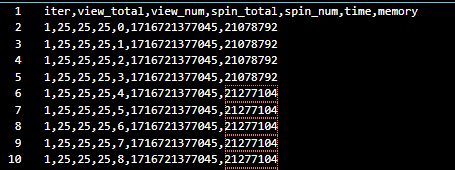
\includegraphics[width=0.4\textwidth]{images/MVC_Start}
		\caption{Output awal MVC}
		\label{fig:start_mvc}
	\end{figure}
	
	Data ini menunjukkan bahwa program secara iteratif membuat dan membuang sejumlah tampilan dan spinner yang ditentukan, mencatat penggunaan memori dan waktu untuk setiap konfigurasi. Seperti yang diilustrasikan figure 9, dalam iterasi 1 dengan 25 tampilan dan 25 spinner, penggunaan memori konsisten pada 24.753.584 byte dan total time sebanyak 1.716.721.377.045 millisec, sedangkan pada iterasi 12 dengan 100 tampilan dan 100 spinner, penggunaan memori stabil sekitar 215.465.472 byte dan total time sebanyak 1.716.722.517.068 millisec. Total waktu untuk testing app tersebut adalah 19.09346 menit.
	
	\begin{figure}[h]
		\centering
		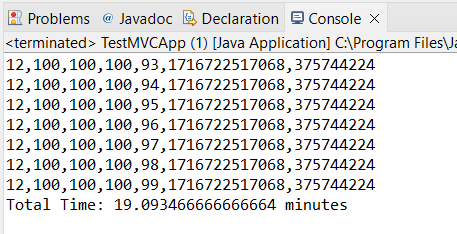
\includegraphics[width=0.5\textwidth]{images/MVC_END}
		\caption{Output akhir MVC}
		\label{fig:end_mvc}
	\end{figure}
	
	\vspace{3cm}
	
	\subsection{Pola Arsitektur MVVM}
	Pada figure 10, diilustrasikan hasil output untuk setiap baris dalam file CSV mewakili satu pengukuran, termasuk kolom untuk nomor iterasi (iter), jumlah total tampilan yang dibuat (\textit{view total}), nomor tampilan (\textit{view num}), jumlah total spinner yang dibuat (\textit{spin total}), indeks spinner dalam total (\textit{spin num}), waktu sistem dalam milidetik saat pengukuran diambil (time), dan memori yang digunakan oleh Java Virtual Machine (JVM) pada saat pengukuran (memory). 
	
	\begin{figure}[h]
		\centering
		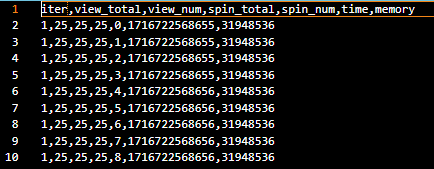
\includegraphics[width=0.4\textwidth]{images/StartMVVM}
		\caption{Output awal MVVM}
		\label{fig:start_mvvm}
	\end{figure}
	
	Mirip dengan penjelasan MVC, program MVVM ini secara iteratif membuat dan membuang sejumlah tampilan dan spinner yang ditentukan, mencatat penggunaan memori dan waktu untuk setiap konfigurasi.  Pada figure 11, kita bisa lihat dalam iterasi 1 dengan 25 \textit{view} dan 25 \textit{spinner}, penggunaan memori konsisten pada 20.872.144 byte dan total time sebanyak 1.716.722.568.656 millisec sedangkan pada iterasi 12 dengan 100 \textit{view} dan 100 \textit{spinner}, penggunaan memori konsisten pada 379.372.808 dan total time sebanyak 1.716.723.718.948 millisec. Total waktu untuk testing app tersebut adalah 19.26506 menit.
	
	\begin{figure}[h]
		\centering
		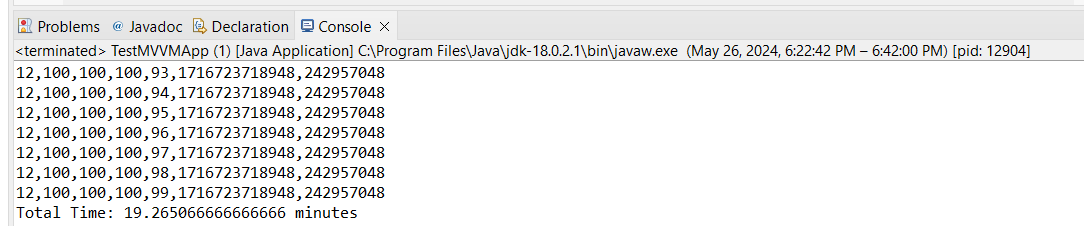
\includegraphics[width=0.5\textwidth]{images/ENDMVVM}
		\caption{Output akhir MVVM}
		\label{fig:end_mvvm}
	\end{figure}
	
	\subsection{Perbandingan MVC dan MVVM}
	Perbandingan hasil testing MVC dan MVVM terbagi menjadi 4 perbandingan yaitu: \textit{View to total time, View to total memory, Spin to total time,} dan \textit{Spin to total memory}.
	\subsubsection{Perbandingan \textit{View to total time}}
	Hasil perbandingan \textit{View to Total Time} adalah MVVM lebih unggul dan cepat untuk menangani peningkatan jumlah \textit{view} dibandingkan dengan MVC. Hal ini terlihat pada average time taken untuk setiap \textit{view} dalam MVVM (1716723180500 millisec) lebih rendah daripada MVC (1716721982868 millisec) yang dapat dilihat pada figure 12.
	
	\begin{figure}[h]
		\centering
		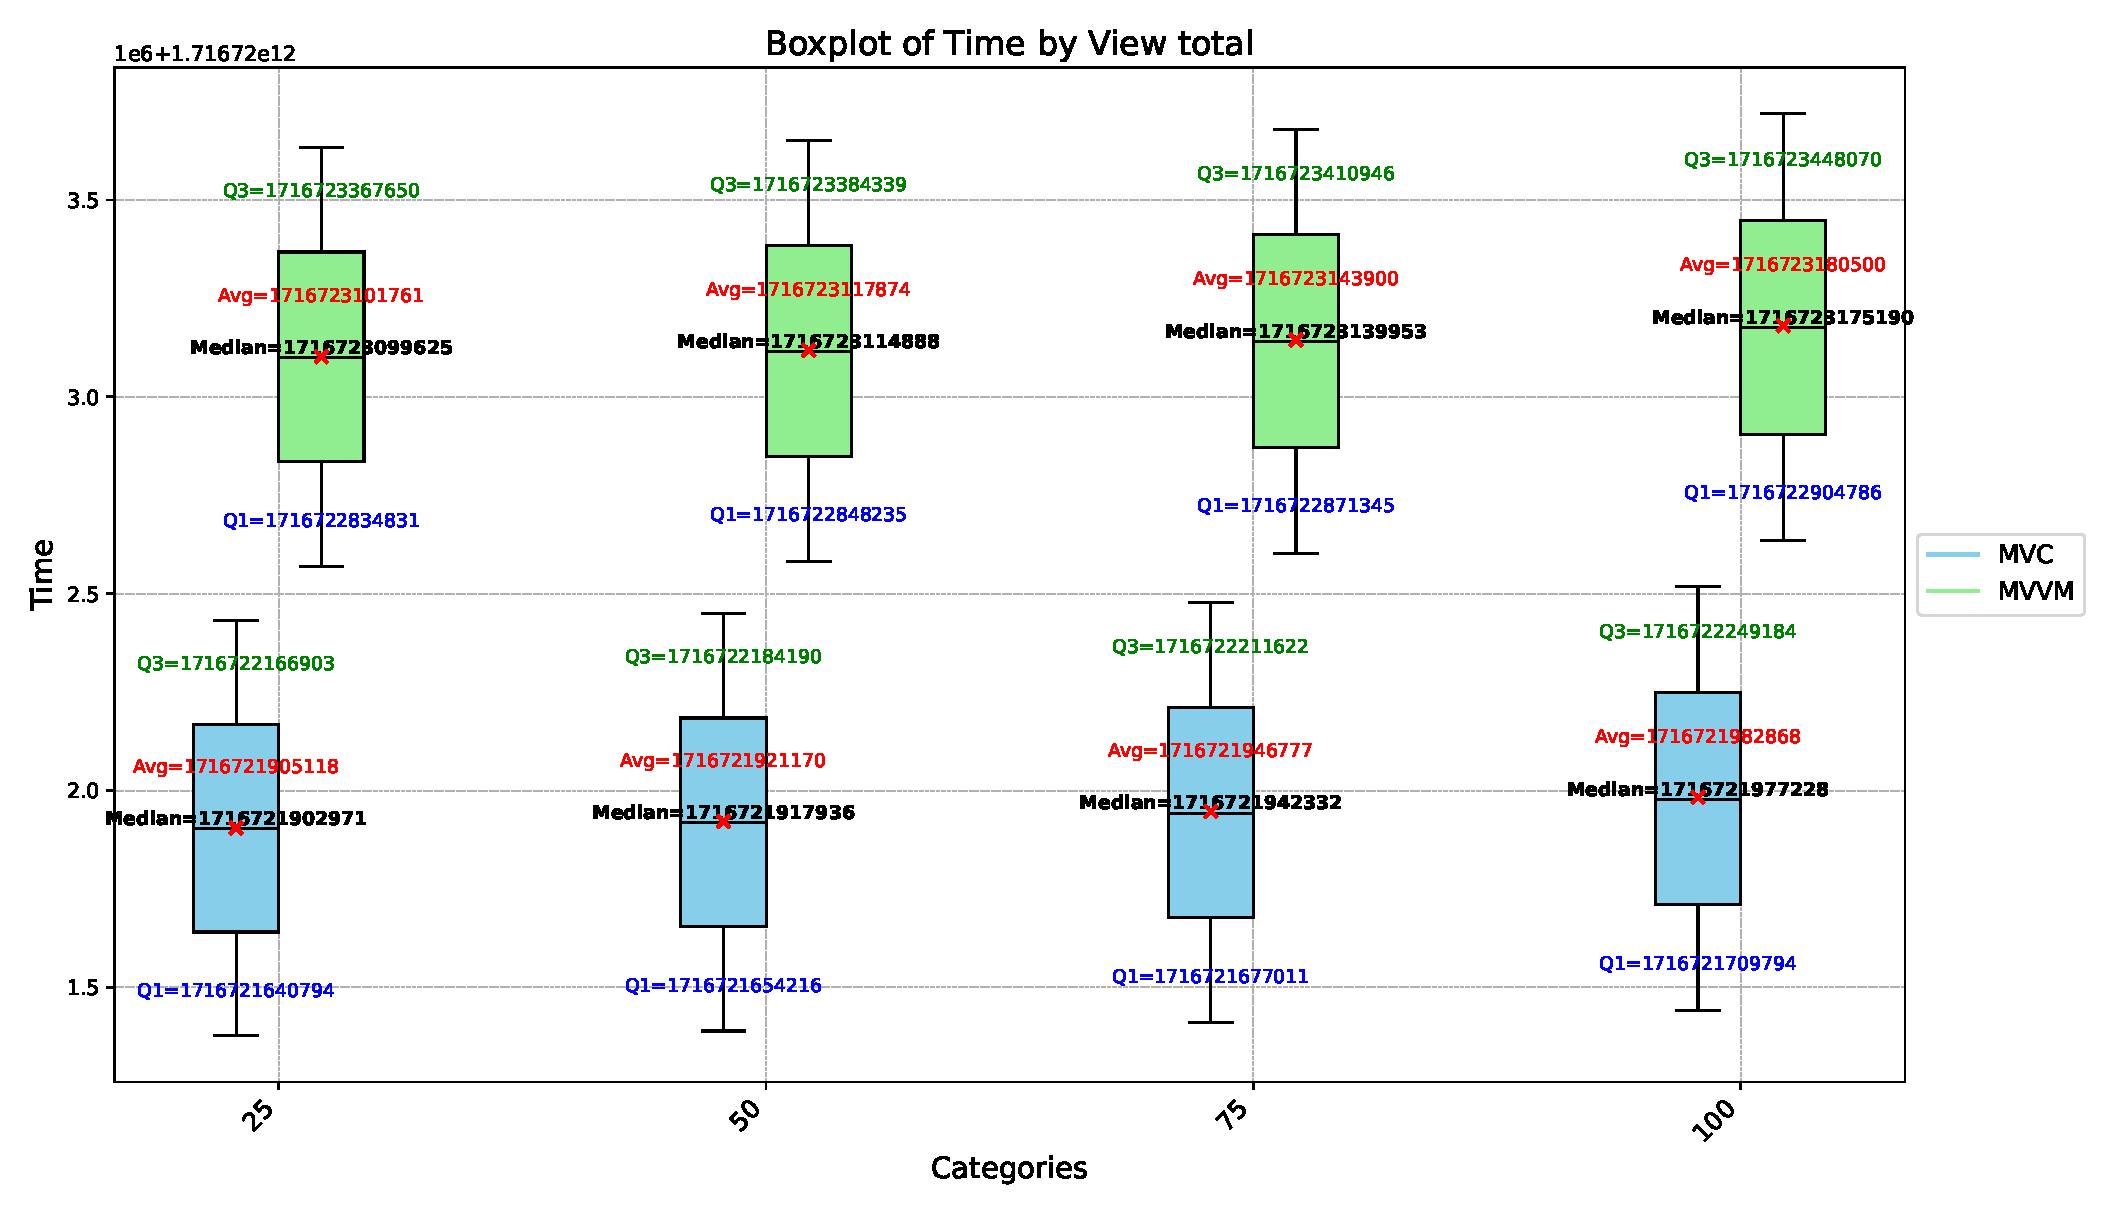
\includegraphics[width=0.5\textwidth]{../mvc-mvvm/plot_view_total_time.pdf}
		\caption{Perbandingan \textit{Total View to Total Time}}
		\label{fig:total_view_to_total_time}
	\end{figure}
	
	\subsubsection{Perbandingan \textit{View to total memory}}
	Hasil perbandingan \textit{View to Total Memory} adalah MVVM lebih unggul dalam penggunaan memori berdasarkan jumlah \textit{view} dibandingkan dengan MVC. Hal ini terlihat pada average memori untuk setiap \textit{view} dalam MVVM (182523212 byte) lebih rendah daripada MVC (269571898 byte) serta diilustrasikan pada figure 13.
	\begin{figure}[h]
		\centering
		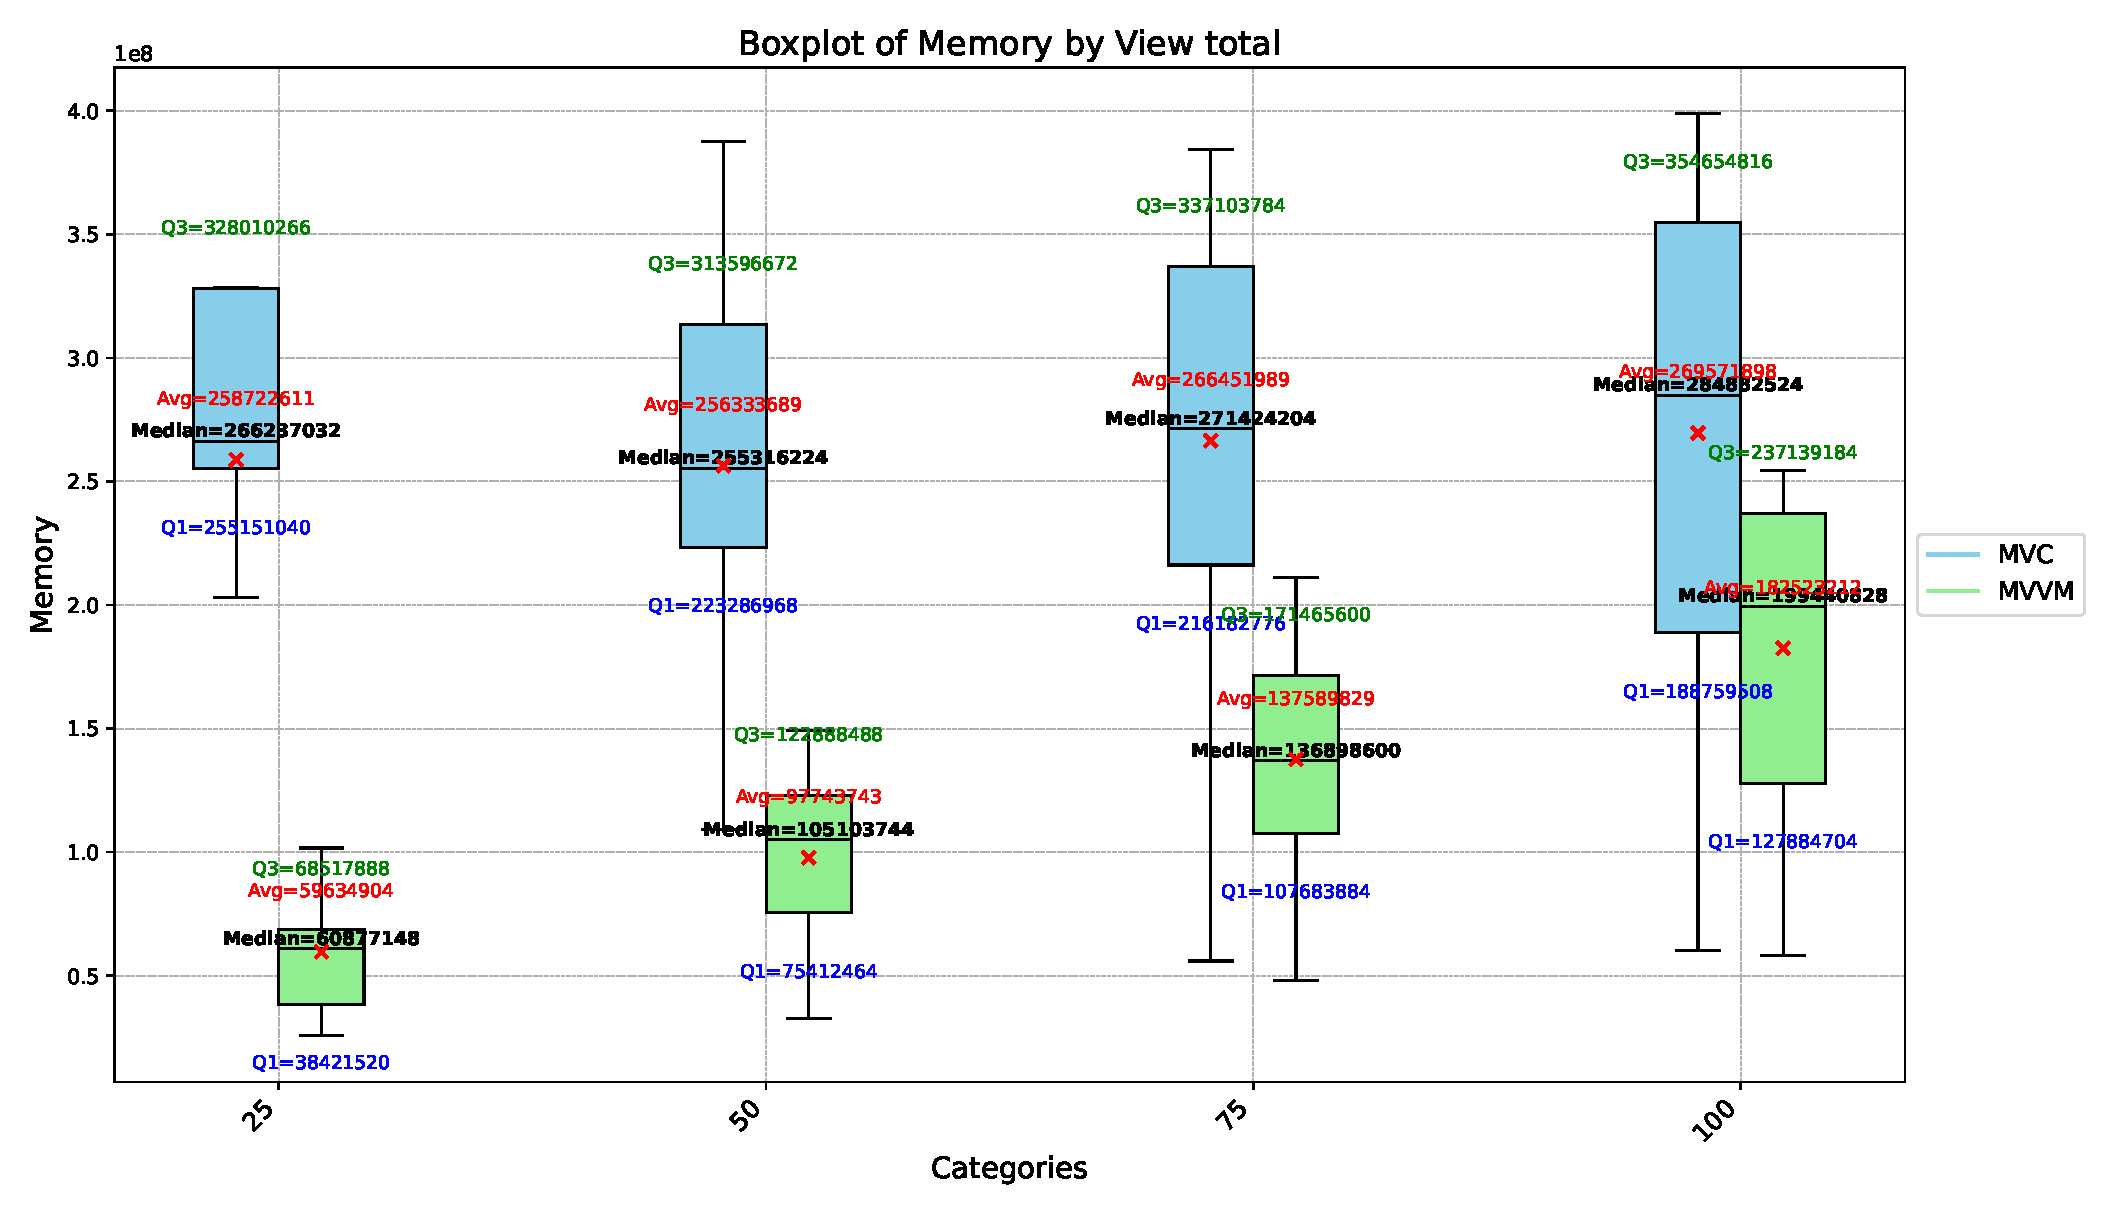
\includegraphics[width=0.5\textwidth]{../mvc-mvvm/plot_view_total_memory.pdf}
		\caption{Perbandingan \textit{Total View to Total Memory}}
		\label{fig:total_view_to_total_memory}
	\end{figure}
	
	\subsubsection{Perbandingan \textit{Spin to total time}}
	Hasil perbandingan \textit{Spin to Total Time} adalah MVC lebih unggul dan cepat untuk menangani peningkatan jumlah \textit{spin} dibandingkan dengan MVVM. Hal ini terlihat pada average time taken untuk setiap \textit{spin} dalam MVC (1716721944593 millisec) lebih rendah daripada MVVM (1716723141670 millisec) yang dapat dilihat pada figure 14.
	
	\begin{figure}[h]
		\centering
		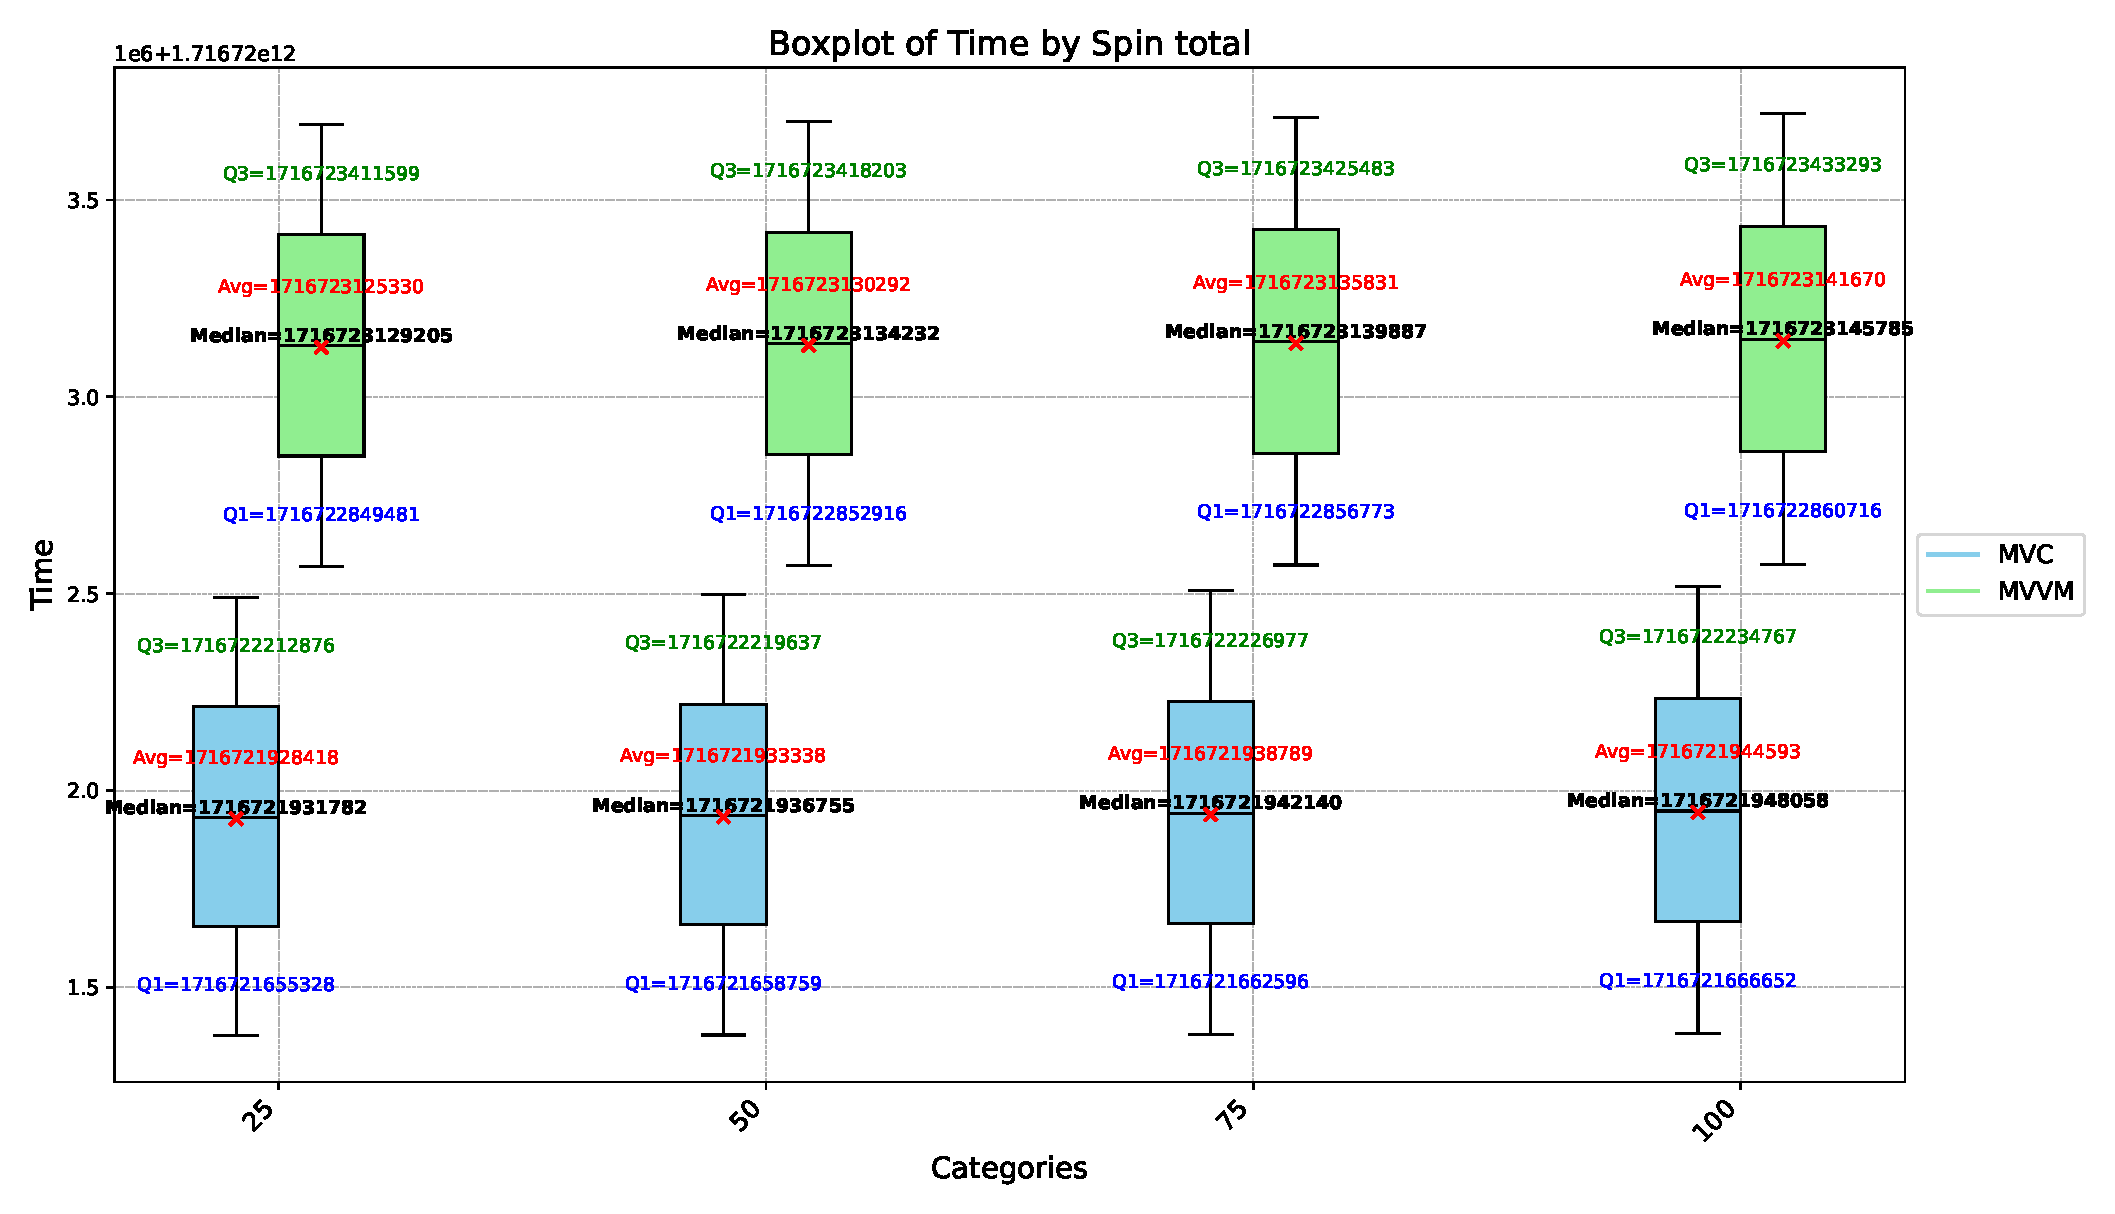
\includegraphics[width=0.5\textwidth]{../mvc-mvvm/plot_spin_total_time.pdf}
		\caption{Perbandingan \textit{Total Spin to Total Time}}
		\label{fig:total_spin_to_total_time}
	\end{figure}
	
	\vspace{3cm}
	
	\subsubsection{Perbandingan \textit{Spin to total memory}}
	Hasil perbandingan \textit{Spin to Total Memory} adalah MVVM lebih unggul dalam penggunaan memori berdasarkan jumlah \textit{spin} dibandingkan dengan MVC. Hal ini terlihat pada average memori untuk setiap \textit{spin} dalam MVVM (155467091 byte) lebih rendah daripada MVC (315097569 byte) serta diilustrasikan pada figure 15.
	
	\begin{figure}[h]
		\centering
		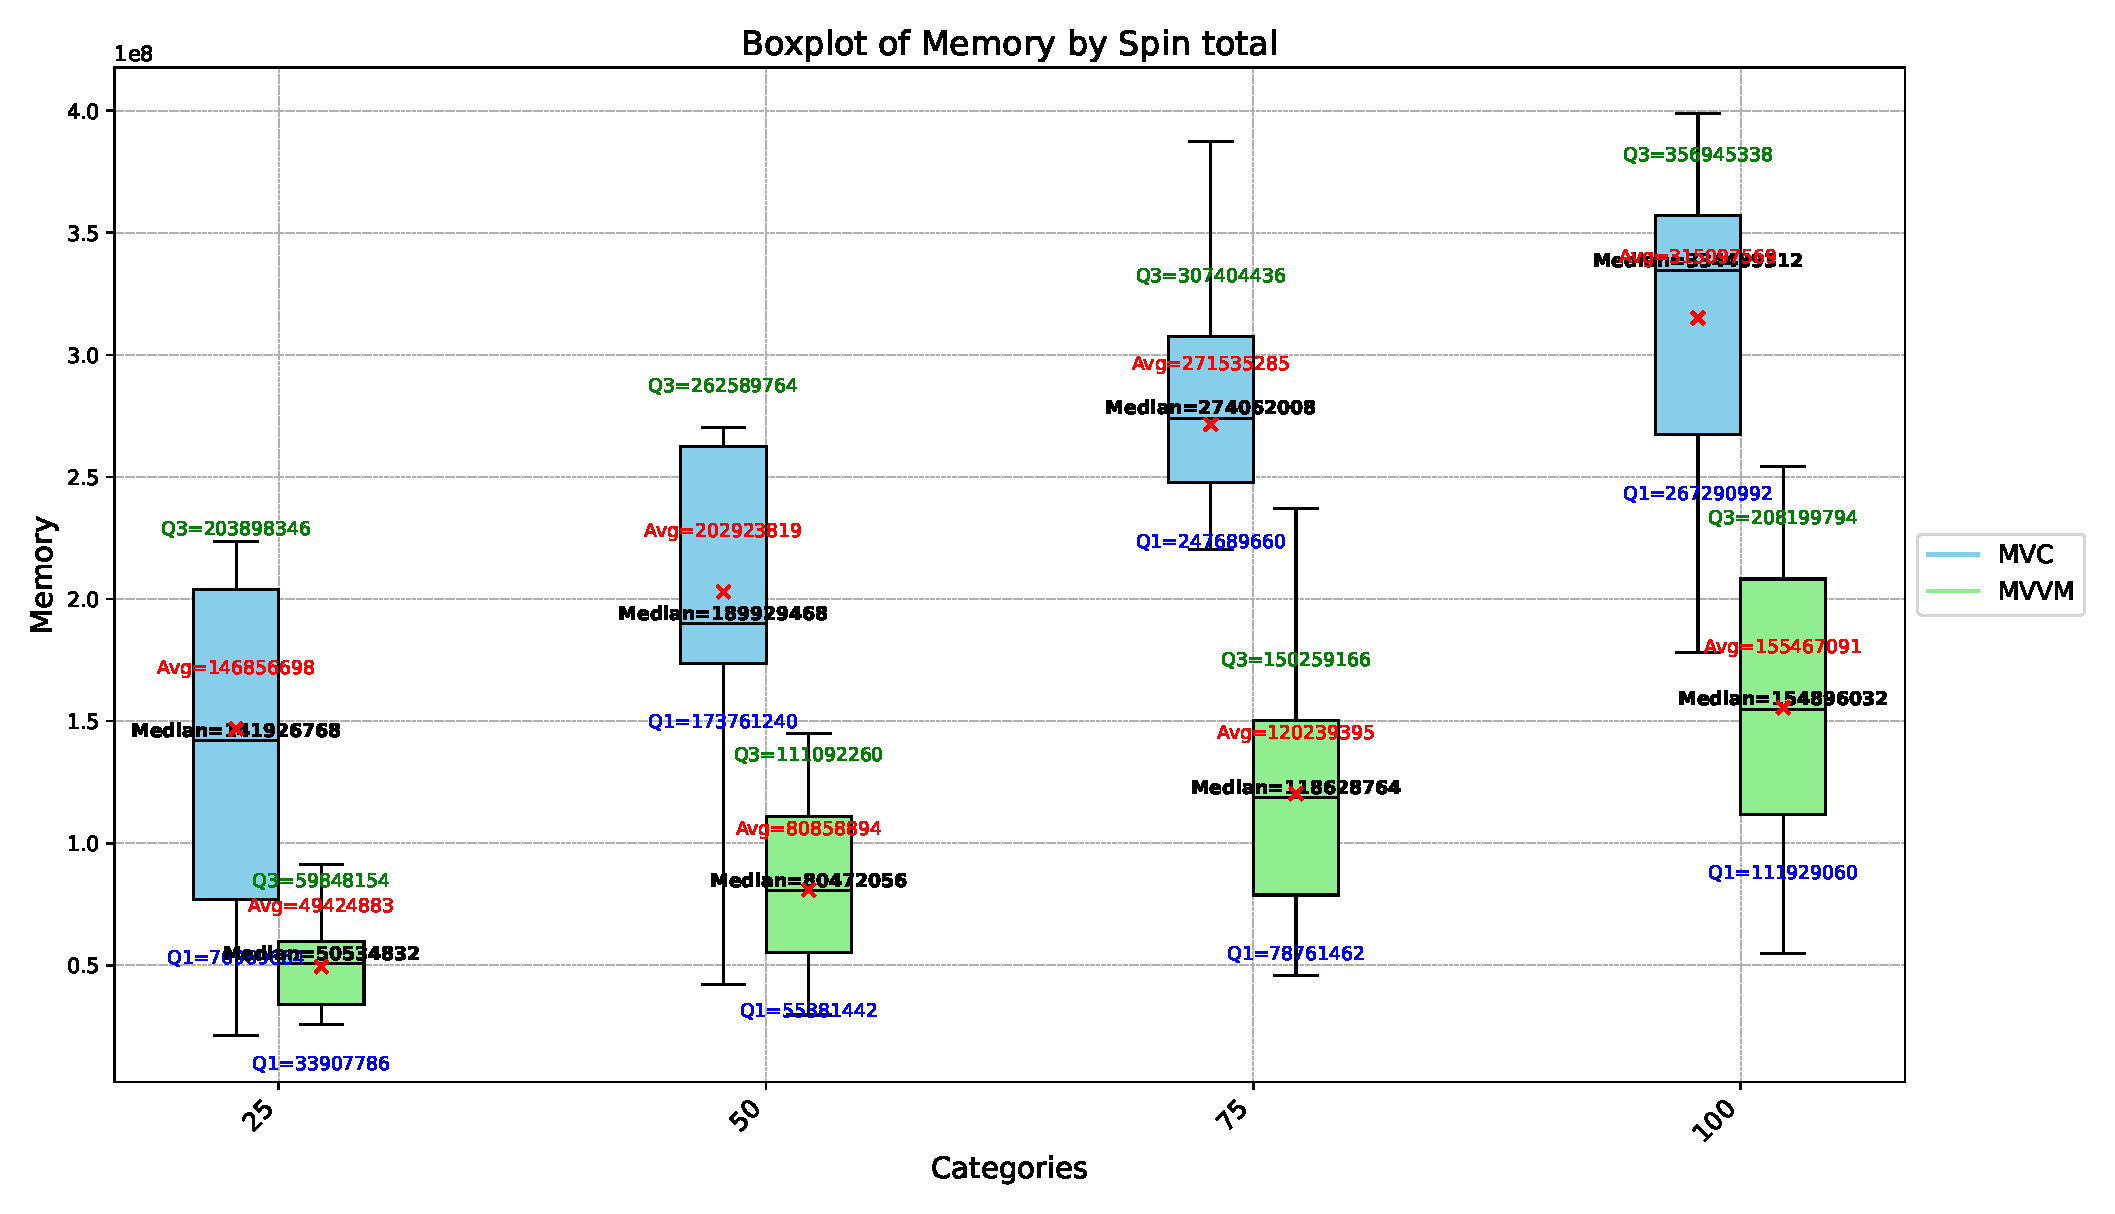
\includegraphics[width=0.5\textwidth]{../mvc-mvvm/plot_spin_total_memory.pdf}
		\caption{Perbandingan \textit{Total Spin to Total Memory}}
		\label{fig:total_spin_to_total_memory}
	\end{figure}
	
	Hasil testing ini adalah MVVM lebih efisien dalam hal waktu dan penggunaan memori saat menangani peningkatan jumlah \textit{view}. Namun, MVC lebih unggul dalam menangani peningkatan jumlah \textit{spin}. Hal yang menarik dari hasil testing ini adalah bahwa alasan mengapa MVC menyelesaikan test dengan total time yang lebih cepat daripada MVVM mungkin disebabkan oleh halnya MVC lebih unggul dalam menangani peningkatan jumlah \textit{spin}.
	
	
	\section{Kesimpulan}
	Kesimpulan yang dapat diambil dari penelitian ini adalah dalam hal kecepatan eksekusi, arsitektur \textit{Model-View-ViewModel} (MVVM) cenderung lebih cepat dibandingkan dengan \textit{Model-View-Controller} (MVC). Hal ini terlihat dari waktu eksekusi yang lebih konsisten dan efisien dalam menangani operasi yang melibatkan perubahan data pada banyak \textit{view}. Namun, penggunaan memori oleh MVVM lebih tinggi dibandingkan dengan MVC, kemungkinan disebabkan oleh mekanisme data \textit{binding} yang memerlukan lebih banyak sumber daya untuk sinkronisasi antara \textit{ViewModel} dan \textit{View}. Maka dari hasil itu dapat dikatakan bahwa MVC cocok untuk aplikasi yang membutuhkan arsitektur yang lebih sederhana dan mudah dipahami, sementara MVVM lebih cocok untuk aplikasi kompleks dengan banyak interaksi UI dan yang memerlukan efisiensi dalam pemeliharaan dan pengujian.
	
	Kami berharap penelitian ini memberikan wawasan yang bermanfaat tentang kelebihan dan kelemahan masing-masing arsitektur, membantu pengembang untuk membuat keputusan yang lebih baik dalam memilih arsitektur yang tepat untuk proyek mereka, sehingga dapat menghasilkan aplikasi yang lebih efisien dan andal.
	
	\bibliography{reference.bib}
	\vspace{12pt}
	
\end{document}

